\chapter{Introduction}

This chapter will introduce the notion of rephotography, elaborate on the
process of how to make such a photograph and survey existing approaches to
simplify it. These include two applications for mobile operating systems which
will be briefly discussed. Furthermore, a summary of more sophisticated work by
MIT researchers will be given, leading to the problem statement and the goal of
this work.

\section{Overview}

\emph{Rephotography} or repeat photography denotes the retrieval of the precise
viewpoint used for taking a---possibly historic---photograph and capturing
another image from the same spot, ideally with the same camera parameters. This
allows for documentation and visualisation of changes which the scene has
undergone between the two or more captures.  For instance when documenting urban
development, one can present progress of construction, restoration efforts or
changes in the surroundings in a visually striking manner, e.g. by blending the
photographs together.  Figures \ref{fig1} and \ref{fig2} show examples.

\begin{figure}
   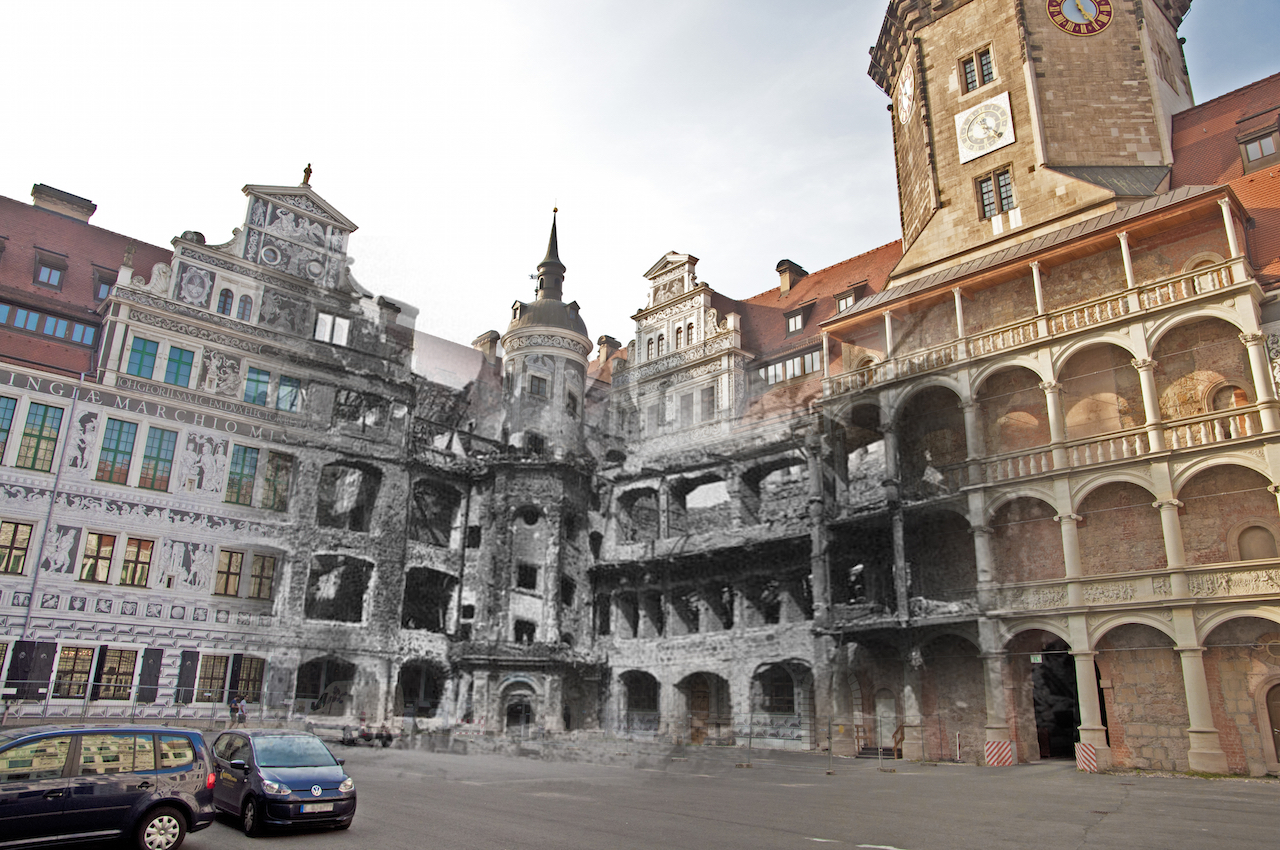
\includegraphics[width=\textwidth]{gfx/1945_2014_Residenzschloss_small.jpg}
   \caption[Residenzschloss Dresden]{Residenzschloss Dresden, destroyed during World War II,
   \textcopyright\ Sergey Larenkov, printed with permission}
   \label{fig1}
\end{figure}

\begin{figure}
   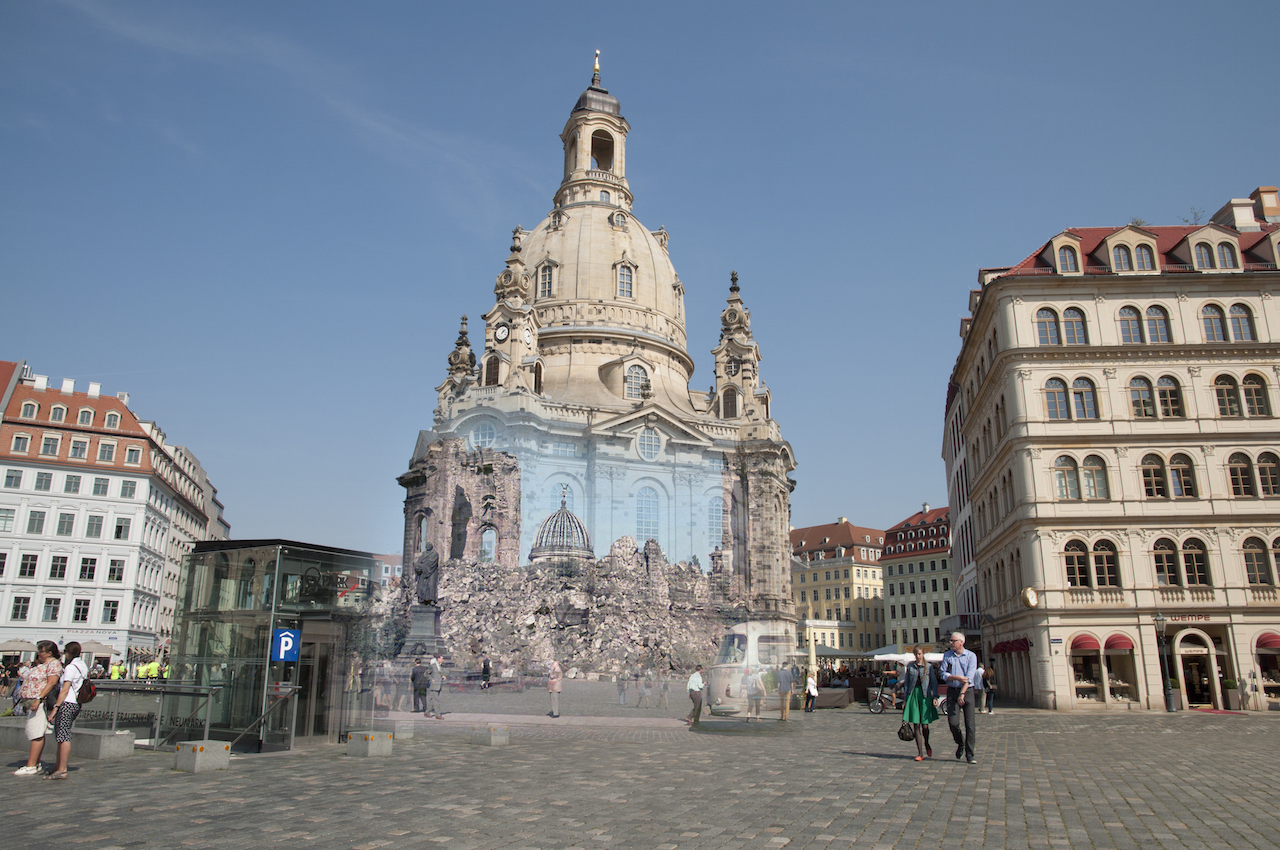
\includegraphics[width=\textwidth]{gfx/1950_2014_Frauenkirche_small.jpg}
   \caption[Frauenkirche Dresden]{Frauenkirche Dresden, destroyed during World War II,
   \textcopyright\ Sergey Larenkov, printed with permission}
   \label{fig2}
\end{figure}

When done manually, the photographer must attempt to find the original viewpoint 
usually by visual inspection of the original image and trying to match the
current camera parameters---camera position, camera rotation, focal length,
possibly principal point---to the original.
The procedure is often carried out by placing the camera on a tripod and
comparing a printout of the original image with what can be seen through the
viewfinder or the camera screen. The number of parameters to match as well as
the difficulty to estimate them purely from comparing two-dimensional images makes the process
error-prone and tedious. Visual acuity and experience of the photographer thus
place limits on the accuracy with which the camera pose of the reference image
can be reconstructed. Some corrections can be done by post-processing the images
and warping the rephotograph with a homography to better match the original.

At the time of writing, few computerised aids are available to the photographer
(see below).  The advancement of mobile phones and tablet computers with
integrated cameras and larger screens presents the opportunity to develop
applications which can assist in this endeavour, moving away from the
traditional trial-and-error approach.  On current digital cameras\footnote{At the time of writing, no commercial manufacturer produces a camera with
   user-modifiable firm- or software. A project at Stanford \citep{Levoy2010}
was discontinued \cite{FrankenCam}} 
this is impossible due to their closed
infrastructure not permitting running user programs. 

\section{Previous Approaches}

\subsection{Mobile Applications}

Two applications have been developed to assist a photographer in taking
rephotographs. For smartphone operating systems,
\emph{rePhoto}\footnote{\url{http://projectrephoto.com/}} and
\emph{Timera}\footnote{\url{http://www.timera.com/Explore}} exist, both
available for Android and iOS devices. These applications support the user by placing a transparent
version of the original image over the current camera image, allowing for easier
alignment. The captured rephotograph is then presented together with the
original image in a blend (c.f. \autoref{fig3}) which can be customized in
\emph{Timera}.

What is characteristical about both of these applications is that the user must still
determine on their own how to actually move the camera. An overlay simplifies
the procedure, eliminating some of the inaccuracy introduced into the manual approach by the
necessity to move the eyes from printout to camera, but it is still the user's
responsibility to determine the necessary motion between the current camera
position and the goal position (that of the original image). 

\subsection{Computational Re-Photography}

A more
sophisticated automated approach was presented in by MIT researchers in
2010. \citet{bae2010} found in preliminary studies that neither a side-by-side
view as would be used in the manual approach, nor a linear blend provided by
the above applications result in accurate rephotographs.

In this setup, the relevant parameters of a historic image's camera are
reconstructed, including the focal length, principal point and the six degrees
of freedom in camera pose. This subsection will give a high-level overview,
while a more in-depth discussion of the relevant concepts is deferred until
\autoref{chapter something}.

The software runs on a laptop connetcted to a digital camera.  After
reconstructing the scene in 3D by use of two images captured by the user, they
are then directed by the software to the desired viewpoint, the user does not
have to find it by themselves.  On the screen, they
are shown the current camera image alongside two arrows indicating in which
direction to move---one for movement in the sensor plane and one for movement
along the optical axis.

\citet*{bae2010} identify five primary obstacles in viewpoint reconstruction of a
historic photograph.
\begin{enumerate}
   \item The necessary camera motion has six degrees of freedom---three for
      translation and three for rotation---which are challenging for the user
      to adjust simultaneously, as changing one parameter will often necessitate
      adjustments for the others to improve the matching. Furthermore, the
      number of degrees of freedom makes it difficult to communicate to the
      user how they must move the camera.
   \item Computing relative translation between two cameras from corresponding
      image points is possible only up to an unknown scale (see
      \autoref{section on projective geometry}), meaning it is impossible to
      determine e.g. if an object viewed by the camera is small and close or
      large and further away. This poses the problem of how to determine if the
      user is close to the desired viewpoint and whether or not they have come
      closer or moved further away over iterations. 
   \item Relative pose estimation from corresponding points fails when the
      motion between the two cameras approaches zero, which is the ultimate goal
      one wishes to achieve. When na\"ivley comparing the current camera image
      to the reference photograph, the estimate for relative rotation and
      translation would become increasingly unreliable as the camera approaches the
      original viewpoint.
   \item Automated computation of relative camera pose will rely on feature
      detection to find correspondences. However, historical images will often
      be vastly different from the current scene. Not only may the scene itself
      have changed considerably, but also the historical image---having been
      taken by a historical camera---may differ in contrast, sharpness and
      colours. Feature detectors may not be able to reliably find
      correspondences when comparing an old with a new photograph.
   \item The calibration data---most importantly, focal length and principal
      point---of the historical camera are often unknown. The calibration data
      is needed for relative pose computation.
\end{enumerate}

Initially, after loading a historical image, the user is instructed to
take two photographs of the scene with a reasonably wide baseline (about
20\textdegree). One of them, termed \emph{first frame} is supposed to be
taken from some distance from the original viewpoint, the \emph{second
frame} should be the user's best eyeballed approximation of it. The wide
baseline allows for a more reliable 3D-reconstrution of the scene used to
tackle problems 2. and 3. 

SIFT features \citep{lowe1999} are computed and matched between the two images.
Given these correspondences, 3D coordinates of the points can be computed. A
selection of these is reprojected into the second frame after which the user
identifies six or more points in the historical photograph corresponding to
these points in the second frame. This allows estimating extrinsic and
intrinsic camera parameters of the historical camera by running an optimisation
algorithm on an initial estimate for relative rotation and translation between
first frame and reference image as well as sensor skew, focal length and
principal point of the historical camera (problem 5.).  The principal point's initial guess
is found again with help of the user who identifies three sets of parallel lines
in the historical image \citep[see][chapter 8.8]{h&z2004}.

The result is that the location of the reference camera relative to the first
camera is known. During the homing process, the current camera frame is compared
to the first frame (not the reference frame, avoiding problem 3.), which avoids
degeneracy due to the wide baseline. Given the locations of the reference camera
and the current frame's camera, each relative to the first frame, one can
compute the location of the reference relative to the current frame and thus
guide the user in the right direction. Hence, the reference photograph is not
needed anymore after this initial step, circumventing problem 4.

During homing, the current camera frame is warped according to the necessary
rotation before being shown to the user, allowing them to focus only on the
translation (problem 1.). This is possible since for rephotography
dealing with structures usually at some distance, the rotation will be small,
otherwise the warped image would be unusable.

A remaining problem (2.) is that the scale of the necessary translation is unknown,
so that only the direction is known. This poses the question of how to determine
whether the user has come closer to the goal or not. It may be feasible to find
the original viewpoint nonetheless, if it was possible to determine at least
when the user reaches it, but this is impossible without further information. On
top of that, it would make for a better user experience if also the distance to
the goal could be communicated.

A key observation in this regard is that the actual scale of the translation is
irrelevant, it is sufficient that there be a way to make the scale consistent
accross iterations. That is, it is unnecessary to know whether the goal is a
specific distance aways, if one can ensure that the translations computed one
after the other can be somehow meaningfully compared. For this, Bae et. al
observe that when triangulating 3D coordinates from corresponding points, their
computed distance from the camera (the first frame) is inversely proportional
to the distance between the cameras. Therefore, in each iteration, the scale of
the world is computed by triangulating correspondences between the first and
current frames. The scale is compared to the scale computed in the initial step
for the first and second frames. Scaling the current translation vector by the
ratio of the two scales makes the length consistent across iterations and
decreasing with the distance to the goal.

The results of this method appear to be very successful, but two main drawbacks
exist.
\begin{itemize}
   \item The prototype is not very convenient, as it requires a (laptop)
      computer and a digital camera to carry out which is impractical for
      spontaneous rephotography.
   \item The application is not available to the public, neither in source nor
      binary form. It is therefore impossible to evaluate adapt for more mobility.
\end{itemize}

\section{Goals of this thesis}

This work's objective can thus be summarised as follows.
\begin{enumerate}
   \item Implement in a prototypal fashion the process from \citep{bae2010} for
      a mobile operating system so it can be run on a smartphone or tablet and
      direct the user in approximate real-time.
   \item Evaluate the approach and attempt to reproduce the results.
\end{enumerate}

For a proof-of-concept application, several simplifying assumptions are made.
Firstly, it is assumed that the ``historic'' photograph is captured with the
same camera as the application is run on and that the camera is calibrated.
Secondly, no strong visual differences between the reference and current scenes
are assumed so that the reference image is accessible to the same feature
detection algorithm without the user manually labelling correspondences. 

The application targets iOS 8 and current hardware, as image processing is
computationally intense, and has been tested on an iPad Air 2.
